\documentclass[psamsfonts]{amsart}

%-------Packages---------
\usepackage{amssymb,amsfonts}
\usepackage{enumerate}
\usepackage[margin=1in]{geometry}
\usepackage{amsthm}
\usepackage{theorem}
\usepackage{verbatim}
\usepackage{graphics}
\usepackage{float}

\newenvironment{sol}{{\bfseries Solution:}}{\qedsymbol}
\newenvironment{prob}{{\bfseries Problem:}}

\bibliographystyle{plain}

\voffset = -10pt
\headheight = 0pt
\topmargin = -20pt
\textheight = 690pt

%--------Meta Data: Fill in your info------
\title{14.15 \\
Networks \\
Problem Set 1}

\author{John Wang}

\begin{document}

\maketitle

Collaborators: Bonny Jain

\section{Problem 1}

\begin{prob}
Consider an undirected tree of $n$ vertices. A particular edge in the tree joins vertices 1 and 2 and divides the tree into two disjoint regions of $n_1$ and $n_2$ vertices.

Show that the closeness centralities $C_1$ and $C_2$ of the two vertices, are related by
\begin{eqnarray}
  \frac{1}{C_1} + \frac{n_1}{n} = \frac{1}{C_2} + \frac{n_2}{n}.
\end{eqnarray}
\end{prob}
\begin{sol}
  First we notice that the sum of the distances of all shortest paths from $1$ $\sum_{j} d_{1j}$ has the following relation with $\sum_{j} d_{2j}$:
  \begin{eqnarray}
    \sum_{j} d_{1j} = \sum_{j} d_{2j} + n_2 - n_1
  \end{eqnarray}

  The above relation follows because the shortest distance from vertex 1 to all vertices in group $n_1$ is exactly one smaller than the shortest distance from vertex 2 to all vertices in group $n_1$. This follows because the only path to from vertex 2 to $n_1$ is through vertex 1 since that edge divides the tree into two disjoint regions. Moreover, by the same logic, the shortest distance from vertex 1 to group $n_2$ is exactly one larger than the shortest distance from vertex 2 to all vertices in group $n_2$. Using this logic, we see that $\sum_{j} d_{1j}$ is simply $\sum_{j} d_{2j}$ corrected for vertex 1 being one closer to all vertices in group $n_1$ and one further from all vertices in group $n_2$. Therefore, we have derived the above relation.

  Now, assuming that $n \neq 0$, we can obtain the following:
  \begin{eqnarray}
    \frac{\sum_{j} d_{1j}}{n} &=& \frac{\sum_{j} d_{2j} + (n_2 - n_1)}{n} \\
    \frac{1}{C_1} &=& \frac{1}{C_2} + \frac{n_2}{n} - \frac{n_1}{n} \\
    \frac{1}{C_1} + \frac{n_1}{n} &=& \frac{1}{C_2} + \frac{n_2}{n}
  \end{eqnarray}

  The final expression is what we wanted to show.
\end{sol}

\section{Problem 2}

Consider an undirected (connected) tree of $n$ vertices. Suppose that a particular vertex in the tree has degree $k$ so that its removal would divide the tree into $k$ disjoint regions, and suppose that the sizes of those regions are $n_1, \ldots, n_k$. 

\begin{prob}
  Show that the unnormalized betweenness centrality of $x$ of the vertex is $x = n^2 - \sum_{m=1}^k n^2_m$.
\end{prob}
\begin{sol}
First, notice that within each of the $k$ disjoint regions, the vertex $x$ does not fall on any shortest path between vertices $i$ and $j$, where $i,j$ are both in the same disjoint region. Without loss of generality, let us examine the $l$th disjoint region. Here, $x$ connects to some vertex $j$ in $l$. However, $j$ is strictly closer than $x$ to any other vertex $i$ in $l$. If this were not the case, then there must be some path from $x$ to $j$ which does not pass through $j$, but this is impossible because this path would lead to a closed loop (and there are no closed loops in trees).

It is obvious, then, that no shortest paths between two vertices in $l$ will pass through $x$. However, we know that the shortest path for vertex $i$ in one region and $j$ in a different region must pass through $x$ because $x$ is the only vertex which connects these two regions. Deleting $x$ causes the regions to become separated, which implies that $x$ is necessarily the only node connecting these regions and hence is in all shortest paths between these regions.

Thus we see that $x$ is contained in all shortest paths between two nodes $i$ and $j$ unless $i$ and $j$ are in the same region.

Notice that the number of shortest paths between $k$ nodes is $k^2$. It follows that the number of shortest paths which go through $x$ is the total possible number of shortest paths ($n^2$) minus the number of possible shortest paths through each region ($\sum_{m=1}^k n_m^2$). Thus, we find:

\begin{eqnarray}
x = n^2 - \sum_{m=1}^k n^2_m.
\end{eqnarray}
\end{sol}

\begin{prob}
Hence, or otherwise, calculate the betweeness of the $i$th vertex from the end of a line graph of $n$ vertices.
\end{prob}
\begin{sol}
We can apply the theorem that we proved above. Notice that the $i$th vertex has degree 2 and its removal would divide up the line (which is also a tree) into 2 distinct regions. The first region has $i-1$ nodes, while the second region has $n-i$ nodes. This means the betweenness of the $i$th vertex by the above theorem is
\begin{eqnarray}
n^2 - (i-1)^2 - (n-i)^2
\end{eqnarray}
\end{sol}

\section{Problem 3}

\subsection{Problem 3.1}
\begin{prob}
Describe an example of a graph where the diameter is more than three times as large as the average path length.
\end{prob}
\begin{sol}
Consider a star graph, where there is a center vertex, and all other vertices have an edge attached to the center vertex. A graph with a high diameter to average path length ratio is a ring graph with a long tail. Thus, if there is a single path of length $D$ connecting to the center vertex, and all other vertices are connected by a single edge to the center, then it is possible to find $n$ and $D$ such that the diameter is three times as large as the average path length.

To see this, we will provide an upper bound for the average path length. Let us define $D$ as the length of the long path (so we know that the diameter of the graph is also $D$). Now, we know that there are $n-D$ vertices which are connected to the center graph, and we also know that the maximum geodesic length is 2. Thus, we see there are $(n-D)^2$ shortest paths of length 2 in this group.

For all other paths, we know there is a maximum length of $D$. Since there are $n^2$ total possible paths, we can have at most $n^2 - (n-D)^2$ shortest paths of length $D$. Therefore, the average path length can be upper bounded by:
\begin{eqnarray}
  \frac{1}{n^2} \left(2 (n-D)^2 + D(n^2 - (n-D)^2)\right)
\end{eqnarray}

If we want the diameter to be greater than three times the average path length, we only need to set that expression to be less than $D/3$ and solve for possible values of $D$ and $n$.

For instance, if we choose $D = 10$ and $n = 120$ in the star graph with long tail as described, we will have a diameter which is three times as large as the average path length.
\end{sol}

\subsection{Problem 3.2}
\begin{prob}
  Describe how you could extend your construction to produce graphs in which the diameter exceeds the average path length by as large a factor as you like.
\end{prob}
\begin{sol}
  We will use the logic given from above. However, we now have some constant $c$ in place of 3. This means that we want to satisfy the inequality:
  \begin{eqnarray}
    \frac{1}{n^2} \left(2 (n-D)^2 + D(n^2 - (n-D)^2)\right) < \frac{D}{c}
  \end{eqnarray}

  By picking some value of $D$, one can solve for possible values of $n$ which satisfy this inequality or vice versa. Therefore, using the star graph with long tail from the previous question, we can achieve an arbitrary factor for which the diameter exceeds the average path length.
\end{sol}

\section{Problem 4}

I obtained the clustering coefficient by having three nested for loops, where the last for loop iterated over values from the second index' + 1 to the size of the matrix. Then I counted the number of times that there were a pair of adjacent edges, as well a triangle. I found that the clustering coefficient was $0.499$.

To obtain the diameter, I used the Floyd Warshall all pairs shortest path algorithm. I found that the largest distance in the matrix was 5, so the diameter of the graph is 5.

To find the average path length, I took the sum of the Floyd Warshall matrix and divided by the size of the matrix squared minus the size of the matrix (because of the diagonals). I found the average path length was 2.607.

I will show the degree distribution below:
\begin{figure}[H]
  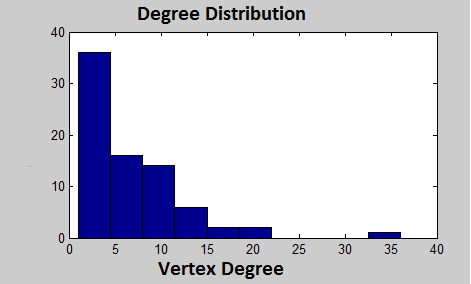
\includegraphics{degree_distribution.png}
\end{figure}

\section{Problem 5}

\subsection{Problem 5.1}
\begin{prob}
  Construct the adjacency matrix for this graph.
\end{prob}
\begin{sol}
  For $m = 5$, the adjacency matrix looks like the following:

  \begin{figure}[H]
    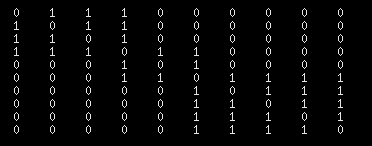
\includegraphics{pset1_adj_matrix.png}
  \end{figure}

  In general, the top left hand corner is a square of size $m-1$ of all ones except for the diagonals which are zero. The bottom right hand corner is a square of size $m$ of all ones except for the diagonals which are zero. The middle of the adjacency matrix consists of a square of size 3 of ones except for the middle element which is zero.
\end{sol}

\subsection{Problem 5.2}
\begin{prob}
Compute the first and second eignvalues of $AD^{−1}$ for $m = 5, 10, 15, 20$.
\end{prob}
\begin{sol}
  First we notice that $D$ is just the sum across each row in the adjacency matrix. Thus, we will use the following matlab code to find the eigenvalues:
  \begin{verbatim}
    D = diag(sum(A));
    eig(A*D^(-1))
  \end{verbatim}

  This gives us the eigenvalues ordered from largest to smallest, and we can simply obtain the first two values in the array to find $\lambda_1$ and $\lambda_2$. Doing this for $m = 5, 10, 15, 20$, we obtain the following:

  \begin{figure}[h!]
  \begin{tabular}{ l | c | c}
    m & $\lambda_1$ & $\lambda_2$ \\
    \hline
    5 & 1.00 & 0.88 \\
   10 & 1.00 & 0.97 \\
   15 & 1.00 & 0.99 \\
   20 & 1.00 & 0.99
  \end{tabular}
\end{figure}
\end{sol}

\subsection{Problem 5.3}
\begin{prob}
  Assume the initial vector is $x(0) = (1, 1 . . . 0, 0 . . . )$ where the value 1 is supported on the first $m$ components. For the cases of $m = 5, 10$, plot the response of $x_1 (k), x_{m+1} (k),$ and $x_{2m} (k)$.
\end{prob}
\begin{sol}
  We can simulate the response by iteratively taking $x(k+1) = AD^{-1} x(k)$. This allows us to plot the responses over time in matlab by taking $x = adinv*x$ and using $x(1), x(m+1), x(2m)$ and plotting the values across time. The results are given below:

\begin{figure}[H]
  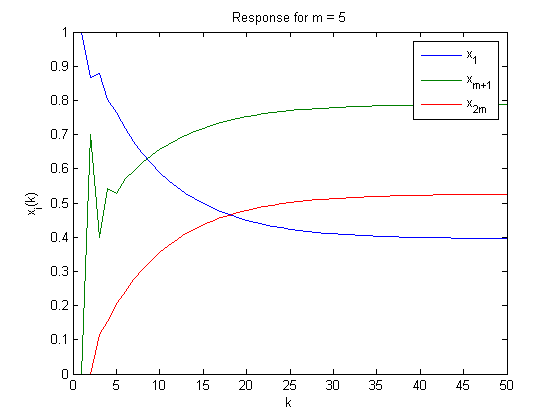
\includegraphics{pset1_m5_response.png}
\end{figure}
\begin{figure}[H]
  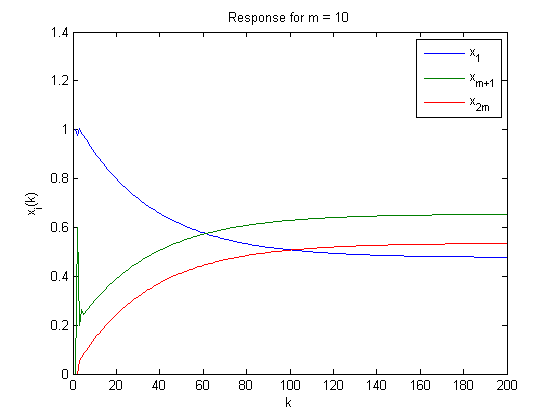
\includegraphics{pset1_m10_response.png}
\end{figure}
\end{sol}

\subsection{Problem 5.4}
\begin{prob}
  What are your observations about the convergence rates of $(AD^{-1})^k$.
\end{prob}
\begin{sol}
  It is clear that the $(AD^{-1})^k$ takes longer to converge when $m$ is larger. We see that for $m=10$ it takes more than twice as long for the responses to converge than when $m=5$. Therefore, we see that convergence slows down with larger $m$. Repeating the same exercise for $m=15$ and $m=20$ gives the same results (though figures are not provided).
\end{sol}

\section{Problem 6}

\subsection{Problem 6.1}
\begin{prob}
Determine the signs of $a$ and $b$ to reflect the behavior of Romeo and Juliet.
\end{prob}
\begin{sol}
  We must have $a > 0$ and $b < 0$. If this is the case, then Romeo will respond positively to Juliet's love, but Juliet will respond negatively to Romeo's love.
\end{sol}

\subsection{Problem 6.2}
\begin{prob}
For what ranges of parameters $a$ and $b$ will Romeo's and Juliet's love fizzle away regardless of where they start?
\end{prob}
\begin{sol}
  We first take the system of equations we are given and notice that exchanging $k+1$ for $k$, we can write $x(k+2) = x(k+1) + a y(k+1)$. Therefore, we can obtain an equation for $x(k+2)$ if we substitute for $y(k+1)$:
  \begin{eqnarray}
    x(k+2) &=& x(k+1) + a b x(k) + a y(k)
  \end{eqnarray}

  However, we know that $x(k+1) = x(k) + a y(k)$ so that $a y(k) = x(k+1) - x(k)$. We can substitute this into the above expression and find:
  \begin{eqnarray}
    x(k+2) &=& 2 x(k+1) + (ab - 1) x(k) \\
    x(k+2) - 2 x(k+1 + (1 - ab) x(k) &=& 0
  \end{eqnarray}

  We can solve this difference equation by obtaining the roots of the characteristic polynomial $p(x) = x^2 - 2x + (1-ab)$. These are obtained from the quadratic equation:
  \begin{eqnarray}
    \lambda &=& \frac{2 \pm \sqrt{4 - 4(1-ab)}}{2} \\
      &=& 1 \pm \sqrt{1 - (1 - ab)} \\
      &=& 1 \pm \sqrt{ab}
  \end{eqnarray}

  Now, we know that Romeo and Juliet's love will fizzle away when $|\lambda| < 1$ for all $\lambda$. However, we know that at least one $\lambda$ will have magnitude greater than or equal to 1, therefore, their love will never go away. Thus, there are no ranges of $a$ and $b$ values for which their love fizzles.
\end{sol}

\subsection{Problem 6.3}
\begin{prob}
  For what ranges of parameters $a$ and $b$ will Romeo's and Juliet's love be forever caught in a cycle of love and hate?
\end{prob}
\begin{sol}
  We simply need to look for values of $a$ and $b$ which cause $\lambda$ to have a non-negative imaginary part. Thus, we need to find values of $a$ and $b$ which make $\lambda = 1 \pm \sqrt{ab}$ imaginary. This occurs whenever $ab < 0$. This occurs when $a < 0, b > 0$ or when $b > 0, a < 0$.
\end{sol}

\subsection{Problem 6.4}
\begin{prob}
  Both Romeo and Juliet were burnt before from loving someone else that does not love them. As a result, their love tomorrow discounts their own love today by a factor of 0.5. Rewrite the model and answer questions 1 and 2.
\end{prob}
\begin{sol}
Now, the more love that either person has, the less they love the other tomorrow. Thus, we can rewrite the model as the following:
\begin{eqnarray}
  x(k+1) &=& -0.5x(k) + a y(k) \\
  y(k+1) &=& b x(k) - 0.5 y(k)
\end{eqnarray}

We can use the same technique we used before. We write $x(k+2) = -0.5 x(k+1) + a y(k+1)$ and subsitute in our equation for $y(k+1)$ to obtain:
\begin{eqnarray}
  x(k+2) = -0.5 x(k+1) + a b x(k) - a (0.5) y(k)
\end{eqnarray}

Now, we substitute the fact that $a y(k) = x(k+1) + 0.5 x(k)$ and obtain:
\begin{eqnarray}
  x(k+2) &=& -0.5 x(k+1) + a b x(k) - 0.5 (x(k+1) + 0.5 x(k)) \\
    &=& - x(k+1) + (ab - 0.5) x(k)
\end{eqnarray}

We can now obtain a characteristic polynomial $p(x) = x^2 + x + (0.5 - ab)$. Solving for the roots, we have:
\begin{eqnarray}
  \lambda &=& \frac{1 \pm \sqrt{1 - 4(0.5 - ab)}}{2} \\
    &=& \frac{1}{2} \pm \sqrt{-\frac{1}{4} + ab}
\end{eqnarray}

For question 1, we keep our original answer and say that $a > 0$ and $b < 0$, which would make Romeo love Juliet more when she loves him, and vice versa for Juliet.

For question 2, we want to find values of $a,b$ such that $\frac{1}{2} > \sqrt{-\frac{1}{4} + ab}$. This occurs when $\frac{1}{2} > ab$ by solving the equality. Thus, we will have eigenvalues less than 1 when $\frac{1}{2} > ab$, so Romeo and Juliet's love will always fizzle when $ab < \frac{1}{2}$.
\end{sol}

\subsection{Problem 6.5}
\begin{prob}
  What happens if both Romeo's and Juliet's love increases by one unit every single time regardless of the actions of the other? Answer questions 1 and 2. Do this for the initial model.
\end{prob}
\begin{sol}
  If Romeo and Juliet's loves increase by 1 regardless of the other's love, then $y(k)$ has a coefficient of $0$ in Romeo's equation and $x(k)$ has a coefficient of $0$ in Juliet's equation. We now have a system of equations as follows:
  \begin{eqnarray}
    x(k+1) &=& x(k) + 1 \\
    y(k+1) &=& y(k) + 1
  \end{eqnarray}

  This is trivial to solve and the resulting system has a slope of 1 for each trajectory $x(k)$ and $y(k)$ regardless of initial condition. If Romeo and Juliet's love increase by 1 in addition to the other dynamics, then we have the system:
  \begin{eqnarray}
    x(k+1) &=& x(k) + a y(k) + 1 \\
    y(k+1) &=& b x(k) + y(k) + 1
  \end{eqnarray}

  We can solve this by using the same technique as before. We know $x(k+2) = x(k+1) + a y(k+1) + 1$ so that $x(k+2) = x(k+1) + a (b x(k) + y(k) + 1) + 1$. Since $a y(k) = x(k+1) - x(k) - 1$, we can substitute and find:
  \begin{eqnarray}
    x(k+2) &=& x(k+1) + ab x(k) + a + 1 + x(k+1) - x(k) - 1\\
      &=& 2 x(k+1) + (ab - 1) x(k) + a
  \end{eqnarray}

  Rearranging, we find that we have:
  \begin{eqnarray}
    x(k+2) - 2 x(k+1) + (1 - ab) x(k) = a
  \end{eqnarray}

  The characteristic polynomial leads to the same roots as before, so we know that $\lambda = 1 \pm \sqrt{ab}$. However, we now have a particular solution $x_p = \frac{a}{1-ab}$.

  We know that the answer to question 1 remains the same. However, when we look at when Romeo and Juliet's love fizzles away, we can see that there is the particular solution. This means that even if $|\lambda| < 1$ for all $\lambda$, the love of Romeo and Juliet will converge to $x_p = \frac{a}{1- ab}$ which is a non-negative value. Therefore, we see that Romeo and Juliet's love will never fizzle away.

\end{sol}


\section{Problem 7}

\subsection{Problem 7.1}

\begin{prob}
  Please go back to the example in the lecture on epidemics and verify the steps outlined above. In that example, we had two equilibria; 0; 1. Verify that 1 is stable for any initial condition in the interval (0; 1] (all points except 0).
\end{prob}
\begin{sol}
  Recall that our system of equations was:
  \begin{eqnarray}
    I(k+1) &=& I(k) + \beta I(k) S(k) \\
    S(k+1) &=& S(k) - \beta I(k) S(k)
  \end{eqnarray}

  We can combine these equations into a single equation by using the fact that $S(k+1) = S(k) ( 1 - \beta I(k) )$ and $I(k) + S(k) = 1$. This means that $I(k+1) = 1 - S(k+1) = 1 - S(k) (1 - \beta I(k))$. Moreover, since $S(k) = 1 - I(k)$, we have that $I(k+1) = 1 - (1 - I(k))(1 - \beta I(k))$. Simplifying this expression, we obtain:
  \begin{eqnarray}
    I(k+1) = (1 + \beta) I(k) - \beta I(k)^2
  \end{eqnarray}

  Now we want to examine the dynamics shifted about the equilibrium at $1$, so let $I(k) = 1 + y(k)$ where $y(k)$ is a small disturbance. We have the equation
  \begin{eqnarray}
    1 + y(k+1) &=& (1 + \beta)(1 + y(k)) - \beta (1 + y(k))^2 \\
        y(k+1) &=& (1 + \beta) y(k) + \beta - \beta ( 1 - 2y(k) + y(k)^2) \\
        y(k+1) &=& (1 - \beta) y(k) - \beta y(k)^2
  \end{eqnarray}

  Now, we can attempt to derive an energy function $V$ for this expression. Take $V(y) = y^2$. It satisfies the requirements of the energy function because $0^2 = 0$ and $y^2 > 0$ for all $y \neq 0$. Now, if we compute $\Delta y$, we have the following:
  \begin{eqnarray}
    \Delta y &=& ((1 - \beta) y - \beta y^2)^2 - y^2 \\
             &=& (1 - \beta)^2 y^2 - 2 \beta (1 - \beta) y^3 + \beta^2 y^4 - y^2 \\
             &=& y^2 \left( -2 \beta + \beta^2 - 2 \beta ( 1 - \beta) y + \beta^2 y^2  \right) \\
             &=& \beta y^2 \left( -2 + \beta - 2 ( 1 - \beta)y + \beta y^2  \right) \\
             &=& - \beta y^2 \left( 2 - \beta + 2 ( 1 - \beta) y - \beta y^2 \right)
  \end{eqnarray}

  Since $0 < \beta < 1$, we know that $2 - \beta > 0$ and that $2 ( 1 - \beta) > 0$. For small values of $y$, all second order terms $y^2$ fall away in comparison to first order terms, so that $(2 - \beta) + 2 ( 1 - \beta) y - \beta y^2 > 0$ for small values of $y$. This means, since $- \beta y^2 < 0$, that $\Delta y < 0$ for small values of $y$. This shows the stability of the equilibrium at $1$.
\end{sol}

\subsection{Problem 7.2}
\begin{prob}
  What can you say about the equilibrium 0?
\end{prob}
\begin{sol}
  We know that the equilibrium at 0 is unstable. This is because we can set $I(k) = 0 + y(k)$ and we will have the equation $y(k+1) = (1 + \beta) y(k) - \beta y(k)^2$. However, for small values of $y$, we know that $y^2$ will be dominated by first order terms. Thus, we see that $y(k+1) \approx (1 + \beta) y(k) > y(k)$. Therefore, we see that $y(k)$ is increasing as $k$ gets larger.

  This shows that $0$ is an unstable equilibrium.
\end{sol}

\subsection{Problem 7.3}
\begin{prob}
  Show that $x(k+1) = - x(k)^3$ is stable at 0.
\end{prob}
\begin{sol}
  Let us substitute $x(k) = 0 + y(k)$ so that we have small perturbations $y(k)$ about 0. Substituting, we have the equation $y(k+1) = - y(k)^3$. Now take the energy function $V(y) = y^2$. As argued from problem 1, this satisfies the requirements of an energy function. Moreover, we have:
  \begin{eqnarray}
    \Delta y &=& (-y^3)^2 - y^2 \\
             &=& y^6 - y^2 \\
             &=& y^2(y^4 - 1)
  \end{eqnarray}

  But we know that $y$ is small such that $y << 1$, so that $y^4 - 1 < 0$. This means that $y^2 ( y^4 - 1) < 0$ which means that $\Delta y < 0$. This shows that the equilbirium at 0 is stable.
\end{sol}

\subsection{Problem 7.4}
\begin{prob}
Is the system $x(k + 1) = -x(k)^2$ stable at 0?
\end{prob}
\begin{sol}
  Yes, we can use the same reasoning to look at an energy function $V(y) = y^2$. We see that the equilibrium about 0 gives the following change in $y$ near 0: $\Delta y = y^2( y^2 - 1) < 0$ which shows stability.
\end{sol}

\subsection{Problem 7.5}
\begin{prob}
  If $f(x)$ is a continuous and convex funcion on $\mathrm{R}$ then show that the iterative algorithm $x(k+1) = x(k) - \gamma f'(x(k))$ converges for $\gamma$ small enough.
\end{prob}
\begin{sol}
  We know that convex functions satisfy the inequality
  \begin{eqnarray}
    f(\alpha x_1 + \beta x_2) \leq \alpha f(x_1) + \beta f(x_2)
  \end{eqnarray}

  Moreover, we know that continuous and convex functions also satisfy the inequality
  \begin{eqnarray}
    f(x_1) - f(x_2) \geq f'(x_1) | x_2 - x_1|
  \end{eqnarray}

  Finally, we know that since $f$ is convex and only has a single global minimum, it is sufficient to show that $f$ converges in order to show that $f$ converges to its minimum. This follows because there is no other equilibrium that it can converge to.

  So, we have the following:
  \begin{eqnarray}
    f(x(k+1)) - f(x(k)) &=& f(x(k) - \gamma f'(x(k))) - f(x(k)) - f(x(k)) \\
                        &\leq& - \gamma |f'(x(k))|^2
  \end{eqnarray}

  Thus it is clear that for small $\gamma$, $f$ will converge.
\end{sol}

\end{document}
